\documentclass[10pt,a4paper]{article}
\usepackage{geometry}
 \geometry{
 a4paper,
 total={170mm,257mm},
 left=20mm,
 top=20mm,
 }


\usepackage[utf8]{inputenc}
\usepackage[spanish]{babel}
\usepackage{graphicx}
\usepackage{wrapfig}
\usepackage{amssymb, amsmath}
\usepackage{tikz}
\usepackage{enumitem}

\title{Calculo Eléctrico Líneas Aéreas}
\author{MakerGarage}
\date{Abril 2021}


\setlength{\parindent}{0cm}


\renewcommand{\thesubsection}{\Roman{subsection}}
\renewcommand{\thesubsubsection}{\alph{subsubsection})}

\begin{document}

\maketitle
\newpage
\tableofcontents
\newpage

\section{Densidad de corriente}
\subsection{Selección del conductor}
Los parámetros que tenemos que conocer son:
\begin{itemize}
    \item $S = \text{Sección [mm]}$
    \item $\text{Hilos de aluminio + Hilos de acero} \xrightarrow{} K$
\end{itemize}
\begin{tabular}{| c | c |}
\hline
Composición & Valor de K \\ \hline
30+7 & 0'916 \\
6+1  & 0'937 \\
26+7  & 0'937 \\
54+7 & 0'95 \\ 
45+7  & 0'97 \\\hline
\end{tabular}


\subsection{Interpolación}
En caso de que mi sección no aparezca en la \textbf{TABLA 11 ITC-LAT07 (mirar aleación de aluminio)} debo interpolar para obtener el valor de la densidad
\\
\subsubsection{Cojo un valor por encima y uno por debajo de mi sección del conductor}
\begin{tabular}{ c c } 
 
 300 \hspace{0.25cm} \xrightarrow{} & 2'15 \\
 400 \hspace{0.25cm} \xrightarrow{} & 1'95 \\
 
\end{tabular}
\\

Selecciono el modo estadística
\\
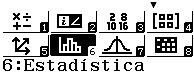
\includegraphics[]{src/01.jpg}\\

Presiono el 2 $y = a+bx$
\\
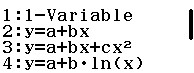
\includegraphics[]{src/02.jpg}\\

Introduzco los valores conocidos de la tabla por arriba y por abajo de mi sección
\\

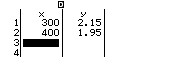
\includegraphics[]{src/03.jpg}\\

Presiono options, bajo y selecciono el 1 \\

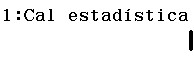
\includegraphics[]{src/04.jpg}\\

Presiono options, bajo y selecciono el 4 
\\

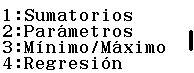
\includegraphics[]{src/05.jpg}\\

Planteo la ecuacion a + Seccion\cdot b
\\
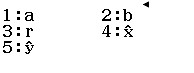
\includegraphics[]{src/06.jpg}\\

Este es el valor de la densidad de corriente interpolada
\\

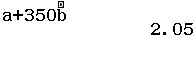
\includegraphics[]{src/07.jpg}\\

\subsubsection{Multiplico el valor de la densidad de corriente ($\delta$) por el de $k$}
$$
\delta_{\text{sección conductor}} = \text{Valor de densidad interpolado} \cdot k
$$
\subsection{Calcular intensidad máxima}
\subsubsection{Intensidad máxima por conductor}
$$
I_{\text{max conductor}} = \delta_{\text{sección conductor}} \cdot S [A]
$$

\subsection{Comprobar Intensidad}
$$
I_{n} = \frac{S_n}{\sqrt{3}\cdot V_n} [A]
$$
ó
$$
I_{n} = \frac{P_n}{\sqrt{3}\cdot V_n\cdot \cos \varphi} [A]
$$
Donde:
\begin{itemize}
    \item $S_n = \text{Potencia aparente en KVA}$
    \item $V_n = \text{Tensión en KV}$
\end{itemize}
\\
\vspace{1cm}
\\

Por último verificamos que se cumple que:
$$
I_n < I_{\text{max conductor}}
$$
\section{Potencia máxima a transportar por densidad de corriente}
$$
P_{max} = \sqrt{3} \cdot V \cdot I_{\text{max conductor}} \cdot \cos{\varphi} \cdot 10^{-3} [MW]
$$
Donde:
\begin{itemize}
    \item $P_{max} = \text{Potencia en MW}$
    \item $V = \text{Tensión en KV}$
    \item $I_{\text{max conductor}} = \text{Corriente en A}$ 
\end{itemize}

\newpage
\section{Aisladores} 
\subsection{Número de aisladores}
$$
n^{\mathrm{o}} \text { aisladores }=\frac{\text { Nivel aislamiento }(\mathrm{mm} / \mathrm{kV}) \cdot \text { Tensión más elevada }(\mathrm{kV})}{\text { Linea de fuga del aislador }(\mathrm{mm})}
$$
Donde:
\begin{itemize}
    \item Nivel de aislamiento = ITC-07 Tabla 14
    \item Tensión mas elevada = ITC-07 Tabla 1
\end{itemize}

\subsection{Perditancia por aisladores}
$$
P=\frac{1000 \cdot w \cdot n}{a_{m}}\cdot 10^{-3} [\frac{kW}{km}]
$$
Donde:
\begin{itemize}
    \item $P = \text{Potencia que se pierde en aisladores en kW/km}$
    \item $w = \text{Pérdida en cada aislador en W}$
    \item $n = \text{Número de aisladores (calculado justo arriba)}$
    \item $a_m = \text{Longitud media de los vanos en m}$
\end{itemize}

$$
G_k=\frac{P(k W / \text { fase })}{\left(\frac{U_{L}}{\sqrt{3}}\right)^{2}} \cdot 10^{-3} [\frac{\text{siemens}}{km}]
$$
Donde:
\begin{itemize}
    \item $G = \text{Perditancia en siemens/km}$
    \item $P = \text{Potencia que se pierde en aisladores en W/km (calculado justo arriba)}$
    \item $U_L = \text{Tensión de línea en kV}$
\end{itemize}
\section{Obtención de los parámetros de línea}
\subsection{Calcular la resistencia}
Calculo la resistencia adecuada a la temperatura de funcionamiento del cable
$$
R_{1}=R_{20} \cdot[1+\alpha \cdot(\theta-20)]
$$
Donde:
\begin{itemize}
    \item $R_{1} = \text{Resistencia a la temperatura de funcionamiento en } \Omega$
    \item $R_{20} = \text{Resistencia que da el fabricante en }\Omega$
    \item $\alpha = \text{Constante = 0.004032 en } \text{\textcelsius}^{-1}$
    \item $\theta = \text{Temperatura de servicio en }\text{\textcelsius}$
\end{itemize}
\\

En caso de tener varios cables (duplex triplex cuadruplex) tengo que dividir la resistencia entre el número de conductores
$$
R_{k}=\frac{R_{1}}{n}
$$
Donde
\begin{itemize}
    \item n es el número de conductores por fase
\end{itemize}
Por último calculo la resistencia total de la línea multiplicando la resistencia kilométrica por la longitud de la línea
$$
R=R_{k} \cdot L
$$
Donde
\begin{itemize}
    \item L es la longitud del conductor en km
\end{itemize}
\subsection{Calcular DMG RMG RMG' (necesarios para calcular la impedancia de la línea)}
Calculo la distancia media entre fases
$$
D M G=\sqrt[3]{D_{1} \cdot D_{2} \cdot D_{3}}
$$
\begin{itemize}
    \item $D_{1} \, D_{2} \,y \,D_{3} \text{ es la distancia entre fases en m}$
\end{itemize}
\\

Calculo el radio del conductor
$$
r = \frac{d}{2}
$$
Donde
\begin{itemize}
    \item $d = \text{Diámetro completo del conductor en mm}$
\end{itemize}
\\

Calculo r'
$$
r^{\prime}=r \cdot e^{-1 / 4}
$$
Calculo el radio medio geométrico
\begin{itemize}
    \item $Duplex = \sqrt{r \cdot D} = RMG$
    \item $Triplex = \sqrt[3]{r \cdot D^2} = RMG$
    \item $Cuadruplex = \sqrt[4]{\sqrt{2} \cdot r \cdot D^3} = RMG$
\end{itemize}
\\
Calculo el radio medio geométrico prima
\begin{itemize}
    \item $Duplex = \sqrt{r \cdot D} = RMG'$
    \item $Triplex = \sqrt[3]{r \cdot D^2} = RMG'$
    \item $Cuadruplex = \sqrt[4]{\sqrt{2} \cdot r \cdot D^3} = RMG'$
\end{itemize}
Donde
\begin{itemize}
    \item $r = \text{Radio del conductor en mm}$
    \item $D = \text{Distancia entre conductores por fase en mm}$
\end{itemize}
\newpage
\subsection{Calcular la impedancia y la capacidad de la línea}
\subsubsection{Impedancia}
\textbf{Inductancia}
\\

Si es línea simple
$$
L_k=2 \cdot 10^{-4} \cdot \ln \frac{D M G}{r^{\prime}}
$$
Si es línea duplex, triplex o cuadruplex
$$
L_k=2 \cdot 10^{-4} \cdot \ln \frac{D M G}{R M G^{\prime}}
$$
Si la línea es de doble circuito
$$
L_k=2 \cdot 10^{-4} \cdot \ln \frac{D M G_{f f}}{D M G_{f}^{\prime}}
$$
$$
D_{12}^{\prime}=\sqrt[4]{D_{12} \cdot D_{12^{\prime}} \cdot D_{1^{\prime} 2} \cdot D_{1^{\prime }2^{\prime }}} 
$$
$$
D_{23}^{\prime}=\sqrt[4]{D_{23} \cdot D_{23^{\prime}} \cdot D_{2^{\prime} 3} \cdot D_{2^{\prime} 3^{\prime}}} 
$$
$$
D_{31}^{\prime}=\sqrt[4]{D_{31} \cdot D_{31^{\prime}} \cdot D_{3^{\prime} 1} \cdot D_{3^{\prime}1^{\prime }}}
$$
$$
D M G_{f f}=\sqrt[3]{D_{12}^{\prime} \cdot D_{23}^{\prime} \cdot D_{31}^{\prime}}
$$
En circuito simplex
$$
D M G_{f}^{\prime}=\left(r^{\prime}\right)^{1 / 2} \cdot\left(D_{11^{\prime}} \cdot D_{22^{\prime}} \cdot D_{33^{\prime}}\right)^{1 / 6}
$$
En circuito duplex o triplex o cuadruplex
$$
D M G_{f}^{\prime}=\left(R M G^{\prime}\right)^{1 / 2} \cdot\left(D_{11^{\prime}} \cdot D_{22^{\prime}} \cdot D_{33^{\prime}}\right)^{1 / 6}
$$
\begin{center}
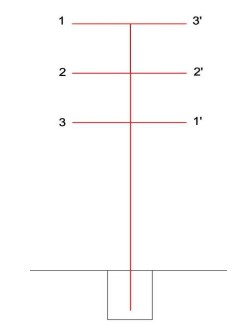
\includegraphics[scale = 0.7]{src/10.jpg}    
\end{center}

\\

$L_k$ = Inductancia en $\frac{H}{km}$
$$
X_k = 2 \cdot \pi \cdot f \cdot L_k 
$$
Donde
\begin{itemize}
    \item $X_k$ = $\frac{\Omega}{km}$
\end{itemize}
$$
X = X_k \cdot L
$$
\begin{itemize}
    \item $L$ = Longitud de la línea en km
\end{itemize}
\newpage
\textbf{Capacidad}
\\
Si es línea simple
$$
C_k=\frac{0,0556}{\ln \frac{D M G}{r}} \cdot 10^{-6}
$$
Si es línea duplex, triplex o cuadruplex
$$
C_k=\frac{0,0556}{\ln \frac{D M G}{R M G}} \cdot 10^{-6}
$$
Si la línea es de doble circuito
$$
C_k=\frac{0,0556}{\ln \frac{D M G_{ff}}{D M G _f}} \cdot 10^{-6}
$$
$C_k = \frac{F}{km}$
\\

\textbf{Susceptancia}
\\
$$
B_k = C_k \cdot 2\cdot \pi \cdot f
$$
$$
B = B_k \cdot L
$$
$B_k$ = $\frac{siemens}{km}$ \\
$L$ = Longitud de la línea en km

\textbf{Perditancia o Conductancia}
\\
$$
G_k=\frac{P(k W / \text { fase })}{\left(\frac{U_{L}}{\sqrt{3}}\right)^{2}} \cdot 10^{-3}
$$
$$
G = G_k \cdot L
$$
$G_k$ = $\frac{siemens}{km}$ \\
$L$ = Longitud de la línea en km
\\

Impedancia
$$
Z = R + jX \, \left[ \Omega \right]
$$

Admitancia
$$
Y = G + jB \, \left[ \text{siemens} \right]
$$
\newpage
\section{Efecto Corona}
$$
U_{C}=\sqrt{3} \cdot 21,2 \cdot m_{c} \cdot \delta \cdot m_{t} \cdot r \cdot n \cdot \ln \left(\frac{D M G}{R M G}\right)
$$
$U_{C}$ : Tensión crítica disruptiva expresada en $\mathrm{kV}$ \\
$m_{c}:$ Coeficiente de rugosidad del conductor $\left(m_{c}=1\right.$ para conductores de superficie lisa) \\ $\left(m_{c}=\right.$ de $0.93$ a $0.98$ para conductores oxidados y rugosos) $\left(m_{c}=\right.$ de $0.83$ a $0.87$ para cables) \\
$m_{t}$ : Coeficiente ambiental (0.8 para tiempo húmedo y 1 para tiempo seco)\\
$r$ : Radio individual del conductor $[\mathrm{cm}]$\\
n: número de conductores por fase. \\
DMG: Distancia media geométrica entre fases [cm] \\
RMG: Radio medio geométrico [cm]\\
$\delta$ : Factor de corrección de la densidad del aire\\
\\
$$
\delta=\frac{273+25}{273+\theta} \cdot e^{\frac{-h}{8150}}\\
$$
$\theta:$ Temperatura $\left[{ }^{\circ} \mathrm{C}\right]$\\
h: Altitud media por donde discurre la línea [m]
\\
\textbf{Hay efecto corona en el caso de que}
$$
U_c < U_s
$$
Siendo $U_s$ la tensión mas elevada 
\\

En caso de existir efecto Corona, procedemos a calcular las pérdidas 
$$
P_{C}=\left(\frac{241}{\delta}\right) \cdot(f+25) \cdot \sqrt{\frac{R M G}{D M G}} \cdot\left(\frac{U_{s}-U_{C}}{\sqrt{3}}\right)^{2} \cdot 10^{-5}
$$
\\

$P_{C}$ es la pérdida de potencia en $\mathrm{kW} / \mathrm{km}$ por fase.\\
$\delta$ es el factor de densidad del aire.\\
$f$ es la frecuencia de la línea en $\mathrm{Hz}$\\
RMG es el radio medio geométrico.\\
DMG es la distancia media geométrica entre fases\\
$U_{s}$ es el valor de la tensión más elevada en $\mathrm{kV}$.\\
$U_{c}$ es el valor de tensión crítica disruptiva en $\mathrm{kV}$.\\
\\
$$
G=\frac{P_{C}}{\left(\frac{U}{\sqrt{3}}\right)^{2}} \cdot 10^{-3}
$$
$P_{C}$ es la pérdida de potencia en $\mathrm{kW} / \mathrm{km}$.fase.\\
$U$ es el valor de tensión nominal de línea en $\mathrm{kV}$.\\
\newpage
\section{Constante de propagación, atenuación y fase}
$$
\begin{array}{l}
\theta=\gamma=\sqrt{\Vec{Z Y}}=\alpha+j \beta \\
\alpha=\text { cte atenuación } \\
\beta=\text { cte fase }
\end{array}
$$
Recordar que la $\sqrt{\Vec{ZY}} = \sqrt{\left|{\Vec{ZY}\right|} }< \frac{angulo}{2}$
\section{Impedancia y potencia característica}
$$
\Vec{Z_{c}}=\sqrt{\frac{\Vec{Z}}{\Vec{Y}}}
$$
Recordar que la $\sqrt{\frac{\Vec{Z}}{\Vec{Y}}} = \sqrt{\left|\sqrt{\frac{\Vec{Z}}{\Vec{Y}}}\right|} }< \frac{angulo}{2}$
$$
P_{c}=\frac{V_{2L}^{2}}{Z_{c}}
$$
Donde:\\
$V_{2L}^{2}$ es la tensión de linea [kV] \\
$P_c$ en MW
\newpage
\section{Circuitos equivalentes}
$V_{2L}$ se saca del enunciado\\
$V_{2F}$ la ponemos como referencia \\
$$I_{F2} =\frac{\frac{P}{3}}{\frac{V_{L2}}{\sqrt{3}}\cdot \cos{\varphi}} [A]$$\\
$$I_{F2} =\frac{\frac{S\cdot cos{\varphi}}{3}}{\frac{V_{L2}}{\sqrt{3}}\cdot \cos{\varphi}}[A]$$\\
Para la intensidad pasamos todo a V W (unidades básicas)
\\

Si la carga es capacitiva el ángulo de la intensidad es positivo, si la carga es inductiva, el ángulo de la intensidad es negativo.\\
\begin{center}
    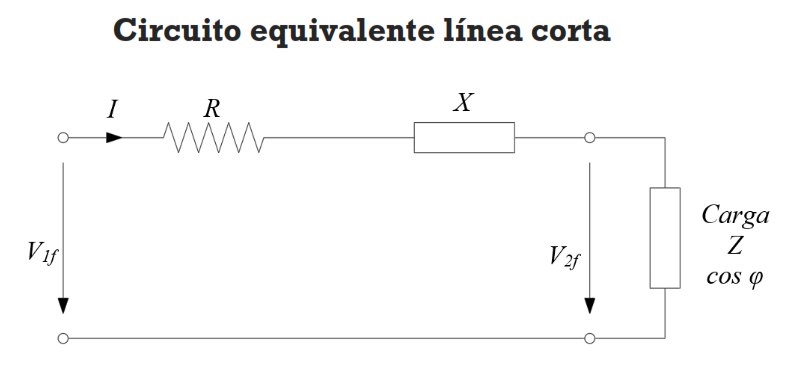
\includegraphics[scale=0.4]{src/Corta.png}
    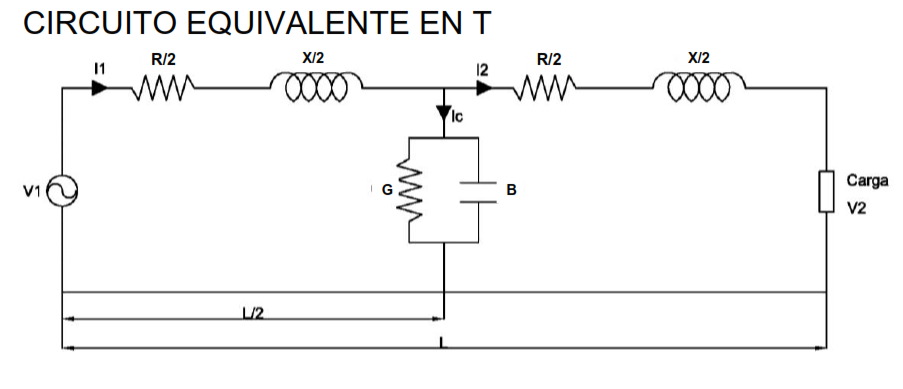
\includegraphics[scale=0.4]{src/Equivalente en T.png}
    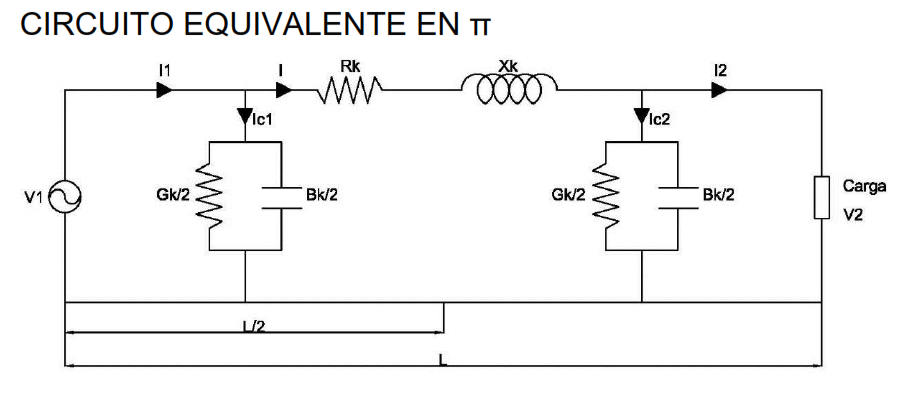
\includegraphics[scale=0.4]{src/Equivalente en pi.png}
    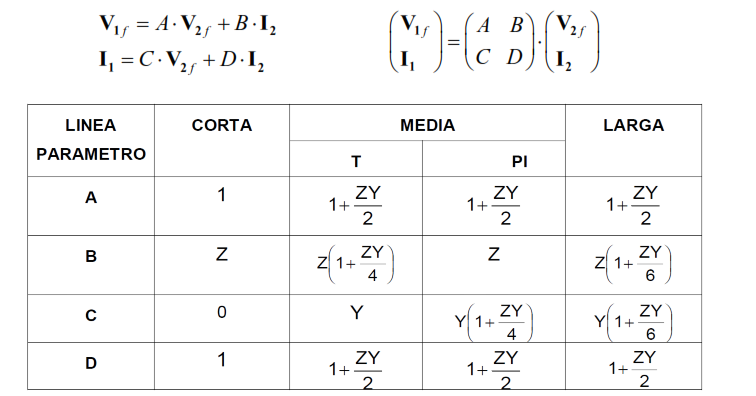
\includegraphics[scale=0.6]{src/tabla.png}
\end{center}
IMPORTANTE QUE LA TENSIÓN ESTE EN V \\
LA Y se pone como $\frac{1}{Y}$ para resolver por circuito a mano
\subsection{Caída de tensión y potencia porcentual}
$$
\Delta V \%=\frac{\left|V_{1}\right|-\left|V_{2}\right|}{\left|V_{2}\right|} \cdot 100 \\
$$
$$
\Delta P \%=\frac{\left|P_{1}\right|-\left|P_{2}\right|}{\left|P_{2}\right|} \cdot 100
$$
$
P_{1}=3\cdot  V_{1F}\cdot 10^3 \cdot I_{1} \cdot \cos \varphi_{1}
$\\
$
P_{2}= \text{Potencia a transportar (enunciado)}
$
\\
Recordad que $\cos \varphi$ es la diferencia entre el ángulo de la tensión de fase y la intensidad de fase.

\end{document}
